\documentclass{chi2009}
\usepackage{times}
\usepackage{url}
\usepackage{graphics}
\usepackage{color}
\usepackage{listings}
\usepackage[utf8]{inputenc}
\usepackage[pdftex]{hyperref}
\hypersetup{%
pdftitle={Your Title},
pdfauthor={Your Authors},
pdfkeywords={your keywords},
bookmarksnumbered,
pdfstartview={FitH},
colorlinks,
citecolor=black,
filecolor=black,
linkcolor=black,
urlcolor=black,
breaklinks=true,
}
\newcommand{\comment}[1]{}
\definecolor{Orange}{rgb}{1,0.5,0}
\newcommand{\todo}[1]{\textsf{\textbf{\textcolor{Orange}{[[#1]]}}}}

\pagenumbering{arabic}  % Arabic page numbers for submission.  Remove this line to eliminate page numbers for the camera ready copy

% remove copyright notice
\makeatletter
\def\@copyrightspace{\relax}
\makeatother

\begin{document}
% to make various LaTeX processors do the right thing with page size
\special{papersize=8.5in,11in}
\setlength{\paperheight}{11in}
\setlength{\paperwidth}{8.5in}
\setlength{\pdfpageheight}{\paperheight}
\setlength{\pdfpagewidth}{\paperwidth}

% use this command to override the default ACM copyright statement 
% (e.g. for preprints). Remove for camera ready copy.
%\toappear{Submitted for review to CHI 2009.}

\title{Natural Language Fact Checker}
\numberofauthors{2}
\author{
  \alignauthor Joshua Kraunelis\\
    \affaddr{University of Massachusetts Lowell}\\
    \affaddr{1 University Ave, Lowell, MA 01852}\\
    \email{jkraunel@cs.uml.edu}
  \alignauthor Wesley Nuzzo\\
    \affaddr{University of Massachusetts Lowell}\\
    \affaddr{1 University Ave, Lowell, MA 01852}\\
    \email{uraniumcronorum@gmail.com}
}

\maketitle

\begin{abstract}
  In this paper we describe the formatting requirements for SIGCHI
  Conference Proceedings, and offer recommendations on writing for the
  worldwide SIGCHI readership.  Please review this document even if
  you have submitted to SIGCHI conferences before, for some format
  details have changed relative to previous years. These include the
  formatting of table captions, the formatting of references, and a
  requirement to include ACM DL indexing information.
\end{abstract}

\keywords{automated fact checking} 

\section{Introduction}

Fact checking is the task of finding evidence to validate or invalidate a given claim. This discipline is most widely applied by journalistic organizations such as newspapers, magazines, and radio/television broadcasters.  However, fact checking isn't limited to journalism, it is also necessary in other venues such as academic publishing.  

Fact checking is either applied either before (ante hoc) or after (post hoc) information has been released, and may be performed by an individual within an organization (e.g. journalist) or by an outside fact checking organization like factcheck.org \cite{factcheck} or Politifact \cite{politifact}.  In any case, whether the fact checking is done for print or broadcast media, by internal or external agents, or for a news article or journal publication, the fact checking is always performed by a human being.  

With more people getting their news from social media outlets such as Facebook and Twitter, there is a need to scale up fact checking to handle the tremendous volume and rate at which stories are disseminated.  In this paper, we propose a system which can verify basic types of claims automatically, without the need for a human fact checker.

\subsection{Related Work}
Researchers at Fullfact.org \cite{babakar_moy_2016} define three main approaches to automated fact checking: reference, machine learning, and context.  The reference approach relies on some official source of information to validate the claim.  The machine learning approach uses some model of how the world works to estimate the likelihood of a claim.  The contextual approach looks at the prevalence of a claim to decide how likely it might be.

Hassan et al. \cite{hassan2015quest} present a system for identifying claims automatically via machine learning.  Their software, ClaimBuster, performs natural language processing tasks such as sentiment analysis, tokenization, part of speech tagging, and entity resolution to classify a sentence as non-factual, unimportant factual, or check-worthy factual.  This system reduces the amount of time spent searching for claims to be validated, though it does not perform the validation itself.  

Ciampaglia et al. \cite{ciampaglia2015computational} take a graph-theoretic approach to automated fact checking.  They encode knowledge from Wikipedia into graph data structures called knowledge graphs that, together, form larger structures called knowledge networks.  They show that traditional graph/network analysis techniques such as shortest path computation can be used to efficiently evaluate the truthfulness of a claim.


\section{Project Description}

The Natural Language Fact Checker employs concepts from two major areas of artificial intelligence: Natural Language Processing and Logic Programming.  The natural language processing component is necessary for the identification and semantic interpretation of individual words or phrases contained within an English sentence (i.e. a claim, in the context of the fact checker).  The semantics of a claim are used to extract zero or more assertions about the claim.  Those assertions are supplied to the logic component.  

\subsection{Natural Language Processing}

This section describes the key techniques, technologies and tools used in the natural language processing component.  

All of the NLP code was implemented using the Python Natural Language Toolkit (NLTK) \cite{nltk}.  We chose to work with NLTK for many reasons, including our familiarity with the Python programming language, the availability of a number of NLP methods, the integration of numerous well known corpora, and the extensive collection of documentation and tutorials available online.
 
For the fact checker, our NLP pipeline consists of the following four steps:

\begin{itemize}
   \item Tokenization
   \item Part-of-speech tagging
   \item Named-entity Extraction
   \item Relation Extraction
\end{itemize}

Tokenization is the process by which a sentence is segmented into smaller pieces (i.e. words, punctuation, etc.).  Many NLP applications employ sentence segmentation to break a larger body of text into separate sentences, then apply tokenization to each sentence.  Our fact checker is designed to process only a single sentence at a time, therefore we have no need for sentence segmentation.  To perform tokenization, we use NLTK's word\_tokenize API, which takes in a single string sentence and produces a list of strings representing the tokens in the sentence.  The word\_tokenize method calls two underlying NLTK tokenization algorithms, TreeBankWordTokenizer and PunktSentenceTokenizer, which perform tokenization using a combination of predetermined regular expressions and a pretrained unsupervised model. Listing \ref{tokList} shows an example of tokenization using NLTK.

\begin{lstlisting}[caption=NLTK Tokenization Example, label=tokList]
>>> from nltk import word_tokenize
>>> word_tokenize(``This is a sentence
 that has been tokenized using NLTK's 
word_tokenize API.'')
['This', 'is', 'a', 'sentence', 'that',
 'has', 'been', 'tokenized', 'using', 
'NLTK', ``'s'', 'word_tokenize', 
'API', '.']
\end{lstlisting}

Part-of-speech tagging is the process of identifying the part-of-speech for a given token.  The NLTK pos\_tag method relies on a pretrained perceptron model to classify a token's part-of-speech based on its context.  The pos\_tag method takes a list of string tokens and produces a list of token-tag pairs.  Each tag is represented as an abbreviation of the part-of-speech, and may include information about plurality, possession, and tense.  A collection of tags is referred to as a tagset.  Listing 2 shows an example of the NLTK pos\_tag capability.

\begin{lstlisting}[caption=NLTK POS Tagger Example, label=tagList]
>>> from nltk import pos_tag
>>> pos_tag(tokens)
[('This', 'DT'), ('sentence', 'NN'),
 ('has', 'VBZ'), ('been', 'VBN'), 
('tagged', 'VBN'), ('using', 'VBG'),
 ('NLTK', 'NNP'), (``'s'', 'POS'), 
('pos_tag', 'NN'), ('API', 'NNP'), 
('.', '.')]
\end{lstlisting}

By default, NLTK uses the UPenn tagset \cite{upenn_tags}.  Table \ref{tableTags} describes the tags shown in the example.

\begin{table}
\begin{center}
\begin{tabular}{ | l l | }
\hline
Tag & Definition \\
\hline
DT & determiner \\
NN & singular noun \\ 
NNP & proper noun \\ 
POS & possessive marker \\
VBG & verb, gerund \\ 
VBN & verb, past participle \\
VBZ & verb, 3rd person singular \\
. & period \\
\hline
\end{tabular}
\caption{Some UPenn Tagset Definitions}
\label{tableTags}
\end{center}
\end{table}

Named-entity extraction is the process of identifying tokens or phrases which refer to named entities within text.  Typical named-entities include people, locations, cardinal numbers, and organizations.  NLTK has several named-entity recognizer APIs, however, we chose to use the NLTK interface to the Stanford Named-Entity Recognizer \cite{stanfordner}.  The Stanford NER is a standalone Java tool that must be installed separately, but may be called from Python code using the NLTK interface.  The Stanford NER uses one or more conditional random field models trained on the CoNLL 2003 eng \cite{conll2003} and MUC 6/7 \cite{muc6} datasets to identify named entities.  The API for the named-entity extractor is similar to the POS tagger - it expects a list of tokens and returns a list of token, tag pairs, where the tags are one of 4 classes: location, person, organization, or other. We created a method that combined the output of the part-of-speech tagger with the output of the named-entity recognizer, in order to preserve the part-of-speech tags which were overridden by the NER (i.e. the NER tags unrecognized tokens with the ``other'' tag).  The results are shown in Listing \ref{lstMerge}.

Relation extraction is the process of determining a relationship between one or more entities.  NLTK provides APIs for relation extraction, however we were not able to get them working to our satisfaction.  Instead of using the provided APIs for relation extraction, we took an approach using regular expressions.  Using the Python re module, We created a series of regular expressions that would match if text indicating a certain relationship was present.

By leveraging NLTK and Stanford's named-entity recognizer, we were able to avoid the time consumings tasks of data annotation and model training. 

\begin{lstlisting}[caption=Merged Tags Example, label=lstMerge]
Original Sentence:

John spent his life breaking barriers,
from defending our freedom as a 
decorated Marine Corps fighter pilot 
in World War II and Korea, to setting
a transcontinental speed record, to 
becoming, at age 77, the oldest human
to touch the stars.

Merged Tags:

[('PERSON', 'John'), ('VBD', 'spent'),
('PRP$', 'his'), ('NN', 'life'), 
('VBG', 'breaking'), 
('NNS', 'barriers'), (',', ','), 
('IN', 'from'), ('VBG', 'defending'),
('PRP$', 'or'), ('NN', 'freedom'),
('IN', 'as'), ('DT', 'a'), 
('JJ', 'decorated'), 
('ORGANIZATION', 'Marine Corps'), 
('NN', 'fighter'), ('NN', 'pilot'), 
('IN', 'in'), ('NNP', 'World'), 
('NNP', 'War'), ('NNP', 'II'), 
('CC', 'and'), ('LOCATION', 'Korea'), 
(',', ','), ('TO', 'to'), 
('VBG', 'setting'), ('DT', 'a'), 
('JJ', 'transcontinental'), 
('NN', 'speed'), ('NN', 'record'), 
(',', ','), ('TO', 'to'), 
('VBG', 'becoming'), (',', ','), 
('IN', 'at'), ('NN', 'age'), 
('CD', '77'), (',', ','), ('DT', 'the'), 
('JJS', 'oldest'), ('NN', 'human'), 
('TO', 'to'), ('VB', 'touch'), 
('DT', 'the'), ('NNS', 'stars')]
\end{lstlisting}
 

\subsection{Logic Programming}

The logical reasoning component takes as input the relations extracted by the NLP component and compares them against its knowledge base in order to find contradictions (proving the claim false) or proofs (proving the claim true).

The logical deduction is mostly handled by PyKE (Python Knowledge Engine). \cite{PyKE} Like Prolog, PyKE uses backward-chaining logic to search for proofs of relations based on given facts and rules of deduction. While it may sound like this can easily be hooked up to the NLP component and the work is done, what PyKE doesn't do (on its own) is \textit{disprove} relations. The solution to this is to search for proofs of relations that contradict the relation to be disproved.

Some of these PyKE rules are simple;
for example, a claim that a player weighs a certain amount is confirmed if the corresponding ``weighs'' relation exists;
but some of them are more complicated, such as the ``heavier'' relation, which requires PyKE to find two ``weighs'' relations and compare their values.

Forming contradictory relations is handled in Python (i.e. outside of PyKE), and the way to do it varies depending on the type of relation. For example, the ``weighs'' relation is contradicted by any ``weighs'' relation with the same player and a different weight. The ``heavier'' relation, on the other hand, is contradicted by a ``heavier'' relation that puts the two players in the opposite order.

Because the ways to find contradictions vary, and because the logic component is meant to be general-purpose, rather than specific to a certain kind of claims, the logic component needs a way to load different logical rules and perform deduction on them in a general way.

For this reason, a class called ``RuleBase'' is created that can be inherited from in order to define new logical systems.
Inheriting from the RuleBase means defining the methods ``provable'' and ``contradicts'', the former of which should return True if the claim is provably true, and False otherwise, and the latter of which should return True if the claim is provably false, and False otherwise.

This class makes no assumption about how the logical rules are implemented; in the case of the sports logic, these rules are defined and implemented using PyKE, but the unit tests for the class ``KnowledgeBase'' are defined in terms of a truth-table logic which does not use any PyKE whatsoever.

The ``KnowledgeBase'' class was intended to be used to store both claims to be proved and disproved, and the knowns these proofs are based on.
In practice, since the knowns used for the sports logic were scraped from Wikipedia, bypassing the NLP component, these knowns were hardcoded as PyKE relations in a ``.kfb'' (knowledge fact base) file.
The claims input by the user in the UI, meanwhile, were not stored in the database at all.
Instead, they were simply evaluated by the database in order to determine the correct truth value.

\subsection{Data}
Due to time constraints, we restricted our fact checker to the domain of American professional basketball.  The reasons for this were many:

\begin{itemize}
\item The domain is well known and recognizable by most people (i.e. even non-basketball fans are likely to recognize an athlete such as LeBron James).
\item The roster information and player physical characteristics do not change frequently, therefore the knowledge we encode is likely to be valid for a long duration (i.e. player height is not likely to change over time).
\item The knowledge we chose to represent is well defined and publicly available from many sources.
\item The number of athletes is static and low enough (30 teams in NBA, 15 players per team) that we were able to represent the complete set of all current NBA players without much effort.
\end{itemize}

In order to encode this knowledge into the logic base, we wrote a Python script that would scrape the roster data from https://en.wikipedia.org/wiki/List\_of\_current\_NBA\_team\_rosters.  The script leveraged BeautifulSoup4 \cite{beautifulsoup}, a Python package that provides an easy to use parser for structured documents such as HTML.  The Wikipedia page was scraped for player team affiliation, player height, player weight, and player age.  The height was represented in meters, weight in pounds, and age as number of years old.  

Each of these characteristics was encoded as a Pyke rule, as shown in Table \ref{tableRules}.  We applied normalization to the player and team names such that all characters were converted to lowercase, special characters (e.g. spaces, hyphens, apostrophes) were replaced with the underscore character, and non-English alphabet characters were replaced with their corresponding English alphabet character (or as close as we could get).  For example, the character é would be replaced by the character e.

\begin{table}
\begin{center}
\begin{tabular}{ | l | }
\hline
Rule \\
\hline 
plays\_for(seth\_curry,dallas\_mavericks) \\
height(mario\_hezonja,2.03) \\
height(jerami\_grant,2.03) \\
weight(thon\_maker,223) \\
age(marshall\_plumlee,24) \\
age(kyrie\_irving,24) \\
plays\_for(rodney\_stuckey,indiana\_pacers) \\
plays\_for(hollis\_thompson,philadelphia\_76ers) \\
age(andre\_iguodala,32) \\
height(brandon\_knight,1.91) \\
\hline
\end{tabular}
\caption{Random Sample of Pyke Rules}
\label{tableRules}
\end{center}
\end{table}


\section{Analysis of Results}

Two of the major evaluation metrics for information retrieval tasks are precision and recall.  Wikipedia defines precision as ``the fraction of retrieved documents that are relevant to the query'' \cite{precision} and recall as ``the fraction of documents that are relevant to the query that are successfully retrieved'' \cite{precision}.  Since our fact checker uses the Stanford NER, we naturally inherit the precision and recall performance of that tool.  

\subsection{Web UI}

\begin{figure*}
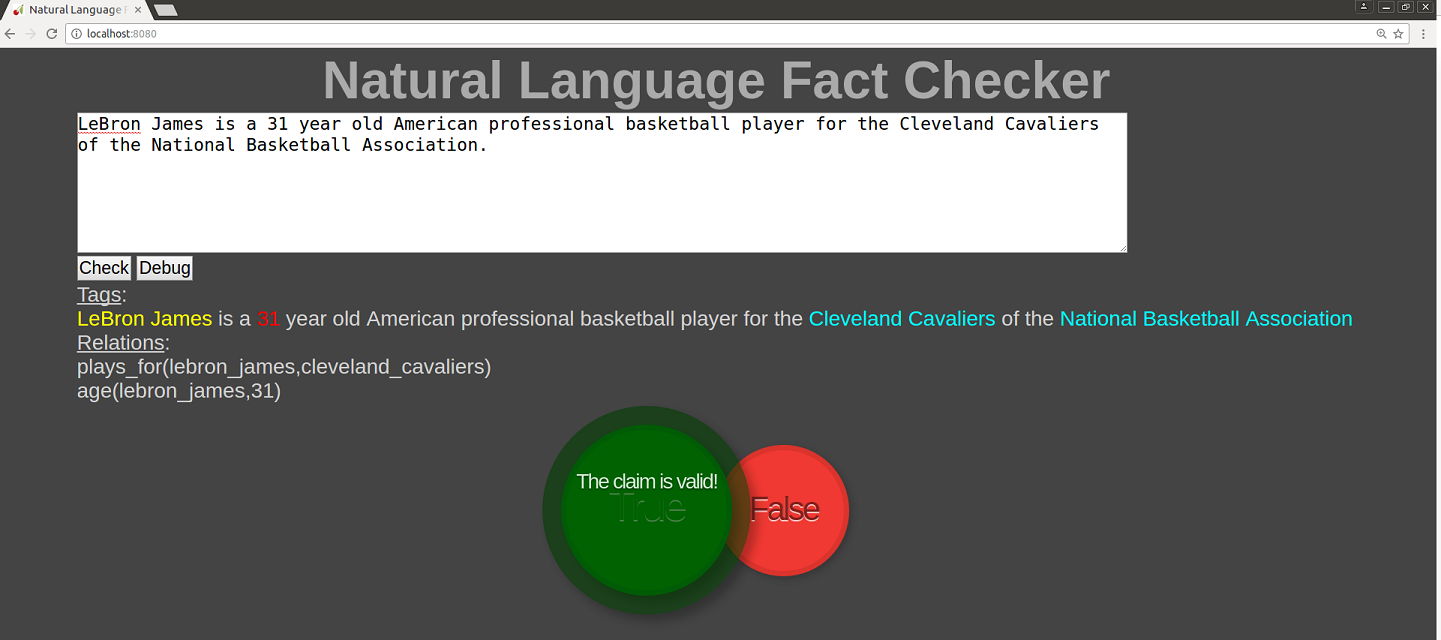
\includegraphics[width=\textwidth,height=9cm]{factcheck}
\caption{Fact Checker Web Interface}\label{imgWeb}
\end{figure*}

While our fact checker is a capable tool for validating claims within the domain we've specified, it is a bit contrived, making it hard to evaluate.  If we were to evaluate our fact checker on a series of randomly picked sports articles, the chance of failure on the relation extraction would likely be very high.  This is due to the fact that we are encoding specific knowledge about player attributes that are unlikely to appear in a story.  In light of this, our major method of evaluating this fact checker was via a web-based user interface, where users could enter a claim and receive feedback from the UI about the truthfulness of the claim.  

To implement the web server, we used the Python CherryPy package.  The server exposed two resources: the main index.html page and a REST API for fact-checking a claim.  The index page contained a text input form, a button for submitting the claim to be fact-checked, a button for enabling/disabling the debug information, and two widgets providing visual feedback of the true/false response of the fact-checker.  

Upon clicking the ``check'' button, the claim that was typed into the text input was posted to the REST API, via an AJAX call, in the form of a URL encoded query string.  The server received and processed the claim, performing the tokenization, part-of-speech tagging, named-entity recognition, and rule extraction in realtime.  The server would then return the debug information, including the tagged entities, and result of the validation to the caller.  The webpage would read the response, update the debug output on screen, and trigger the animation for the corresponding true/false widget.  During the live demonstration on December 7th, the web UI proved to be a valuable way to communicate the effects and abilities of the fact-checker to our audience. Figure \ref{imgWeb} shows a screen shot of the web UI. 

\subsection{Logic Engine Unit Tests}

The logic component defines unit tests for the ``KnowledgeBase'' class, which allows us to verify the correct operation of its features, including some of those that were not used by the web UI. Because the knowledge base depends on a RuleBase in order to work, these tests also test the ``RuleBase'' superclass.

The most noteworthy feature implemented by the logic component but not used by the final web UI is the ability to group claims by their sources and use this grouping to rank these sources in certain ways, such assigning ``reliability'' rankings to the sources based on how the ratio of true:false claims. These features are tested by the ``SourceTest'' tests.

There are three tests:
``KnowledgeTest.testAdd'' checks that the ``addKnown'' and ``addClaim'' methods successfully add claims to the database, and that the truth of a claim to be evaluated is successfully determined based on the claims added using ``addKnown'' (and ignoring claims added using ``addClaim'');
``SourceTest.testTruthRanking'' checks that the method ``truthRanking'', which takes a single source as its argument, correctly returns a tuple representing the ratio of true:false:unknown claims by that source, and that the method ``reliability'' returns a floating point value representing the fraction of provably true or false claims that are true;
finally, ``SourceTest.testContradictions'' checks that the method ``contradictsSelf'' returns True if and only if the source has made contradictory claims.

All of these tests pass.

\section{Discussion}

Given that our fact-checker applied elements of artificial intelligence that weren't necessarily covered in class, we learned a great deal about natural language processing and logic programming while implementing this project.  During the proposal phase, we were both unsure about the feasibility of an automated fact-checker and did a lot of research to identify the available techniques and make a judgment call on how realistic this project might be given the time constraints.  Our research involved reading unassigned chapters of Russell and Norvig, exploring state of the art research in the area of automated fact checking, and evaluating potential software libraries and tools.  

We definitely gained an appreciation for the difficulties involved in natural language processing.  In fact, some of the limiting factors of the project were due to the complexity of the natural language processing component.  For example, the ability to resolve subjects and objects in a verb phrase would enhance the capability of the relation extractor by allowing more sophisticated sentences to be parsed.  This task is doable with NLTK, however, it requires a vast amount of linguistic knowledge to be able to interpret parse trees and other data structures.  Also, our fact-checker only handles single sentence claims, where all of the information we extract is present.  In the real word, authors typically use pronouns in place of proper nouns, employ sarcasm or literary devices, and spread information over multiple sentences.  These factors make the task of information extraction difficult, though there are established techniques to do this.

\subsection{Ethical implications of this work}

Generally, the purpose of fact-checking of this sort is to help people make decisions between opposing viewpoints, based on whether the facts their arguments depend on are accurate.
It can also provide a proxy for judging a politician's trustworthiness, as a politician who relies on a lot of falsehoods likely cannot be trusted as much as one who does not.

This means that users could rely on technology like this to make very important judgments; often judgements that would impact the result of elections.
Because it is important for these judgements to be sound, designers of a technology like this have a clear responsibility to make the meaning of the results clear, and to make the process as transparent as possible.

Ideally, in order to allow users to make their own judgments about the meaning of the results, the AI should not just output either True or False (or some intermediate value), but also should show the basis for those results, including sources.
Our implementation does this to some extent--see the debug mode in the web UI, and note that our knowledge base is capable of keeping track of the sources for its claims.

Another concern for an implementation of an AI like this is how the knowledge base is populated.
For example, if some of the information comes from social media websites or other sources where personal information might be available, this raises the issue of how to handle users' privacy.

Additionally, some potential sources, such as WikiLeaks, have questionable legal and ethical status.
The decision about whether or not to use a source like this could depend on an ethical judgment about whether it is okay to use information that has been distributed in violation of laws--or indeed whether there is an obligation to distribute censored information as an act of civil disobedience.

\section{Conclusions}



\section{Acknowledgments}

The work described in this paper was conducted as part of a Fall 2016 Artificial Intelligence course, taught in the Computer Science department of the University of Massachusetts Lowell by Prof. Fred Martin.

\bibliographystyle{abbrv}
\bibliography{factcheck}

\end{document}
